\subsubsection{Ý tưởng}
Flash Sort là một thuật toán sắp xếp dựa trên việc phân phối các phần tử trong mảng thành các nhóm (lớp), dựa trên giá trị của chúng. Các phần tử sau đó được sắp xếp cục bộ trong từng nhóm và được hợp nhất để tạo thành mảng đã sắp xếp. Thuật toán này hoạt động hiệu quả với mảng có sự phân bố đồng đều. \cite{flashsort1}

\subsubsection{Mã giả}

\begin{algorithm}[H]
\caption{Flash Sort}
\begin{algorithmic}[1]
\Procedure{FlashSort}{$arr, n$}
    \State \textbf{Input:} Mảng $arr$ gồm $n$ phần tử
    \State \textbf{Output:} Mảng $arr$ được sắp xếp
    
    \State \textbf{Bước 1: Phân loại (Classification)}
    \State Tìm giá trị nhỏ nhất $A_{\text{min}}$ và lớn nhất $A_{\text{max}}$ trong mảng $arr$
    \State Tính số nhóm $m \gets \lfloor 0.45 \cdot n \rfloor$
    \State Khởi tạo mảng đếm $L[1..m]$ với giá trị ban đầu là 0
    \For{$i \gets 1$ \textbf{to} $n$}
        \State Xác định nhóm $k_i \gets \lfloor (m - 1) \cdot \frac{arr[i] - A_{\text{min}}}{A_{\text{max}} - A_{\text{min}}} \rfloor$
        \State Tăng $L[k_i]$ lên 1
    \EndFor
    
    \State Tính ranh giới của từng nhóm
    \For{$j \gets 2$ \textbf{to} $m$}
        \State $L[j] \gets L[j] + L[j-1]$
    \EndFor
    
    \State \textbf{Bước 2: Phân phối (Permutation)}
    \State Hoán đổi các phần tử để phân phối chúng vào đúng nhóm
    \State Duyệt từng phần tử, đưa phần tử vào vị trí thích hợp dựa trên nhóm $k_i$
    
    \State \textbf{Bước 3: Sắp xếp từng nhóm (Sorting)}
    \For{$j \gets 1$ \textbf{to} $m$}
        \State Sử dụng thuật toán sắp xếp cục bộ (e.g., \textit{Insertion Sort}) để sắp xếp các phần tử trong nhóm $j$
    \EndFor
\EndProcedure
\end{algorithmic}
\end{algorithm}

\subsubsection{Ví dụ}

Giả sử chúng ta có mảng ban đầu: $[42, 17, 93, 58, 21, 76, 34]$. Dưới đây là các bước thực hiện Radix Sort minh họa bằng hình ảnh:

\begin{enumerate}
    \item Tìm giá trị nhỏ nhất và lớn nhất trong mảng và số lượng Bucket:
    \begin{figure}[H]
        \centering
        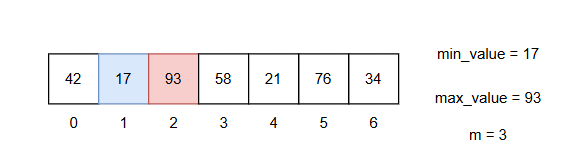
\includegraphics[width=0.7\textwidth]{img/flash_sort/1.png}
        \caption{Minh họa FlashSort-1}
    \end{figure}
    
    \item Tạo mảng \textbf{L} chứa số lượng phần tử trong từng nhóm, duyệt từng phần tử để xác định nhóm của phần tử đó bằng công thức $\lfloor (m - 1) \cdot \frac{arr[i] - A_{\text{min}}}{A_{\text{max}} - A_{\text{min}}} \rfloor$:
    \begin{figure}[H]
        \centering
        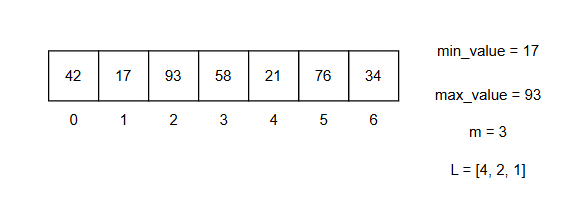
\includegraphics[width=0.7\textwidth]{img/flash_sort/2.png}
        \caption{Minh họa FlashSort-2}
    \end{figure}
    
    \item Thực hiện công dồn ở mảng \textbf{L} để tính ranh giới của các Bucket: 
    \begin{figure}[H]
        \centering
        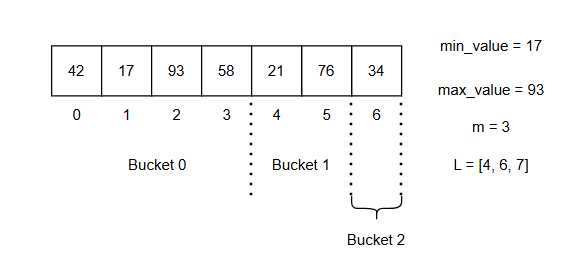
\includegraphics[width=0.7\textwidth]{img/flash_sort/3.png}
        \caption{Minh họa FlashSort-3}
    \end{figure}
    
    \item Tiếp theo là phân phối phần tử vào đúng Bucket, ta duyệt phần tử đầu tiên để tính giá trị $k$ của phần tử đó:
    \begin{figure}[H]
        \centering
        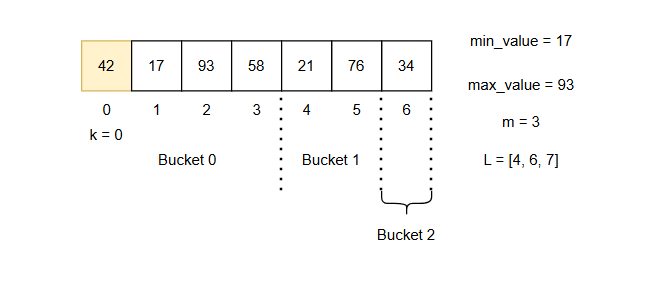
\includegraphics[width=0.7\textwidth]{img/flash_sort/4.png}
        \caption{Minh họa FlashSort-4}
    \end{figure}
    
    \item Giảm giá trị $L[k]$ đi 1 sau đó dưa phần tử vừa tính giá trị $k$ vào vị trí cuối cùng của Bucket $k$, và lưu lại phần tử tại vị trí bị thay thế vào biến tạm thời:
    \begin{figure}[H]
        \centering
        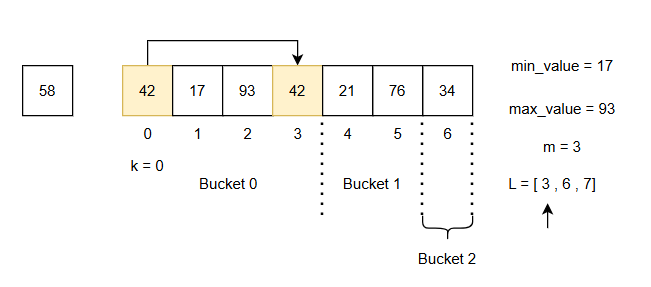
\includegraphics[width=0.7\textwidth]{img/flash_sort/5.png}
        \caption{Minh họa FlashSort-5}
    \end{figure}
    
    \item Tương tự ta làm lại các bước trên đối với phần tử lưu trong biến tạm đến khi tất cả phần tử đều vào đúng Bucket của nó:
    \begin{figure}[H]
        \centering
        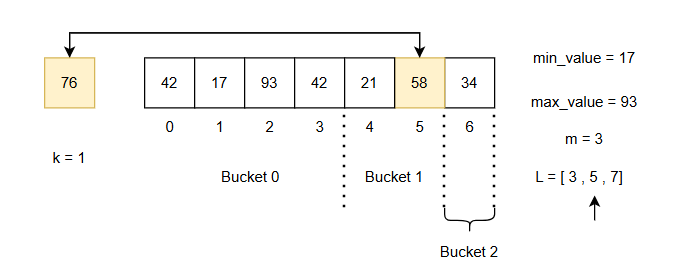
\includegraphics[width=0.7\textwidth]{img/flash_sort/6.png}
        \caption{Minh họa FlashSort-6}
    \end{figure}
    
    \begin{figure}[H]
        \centering
        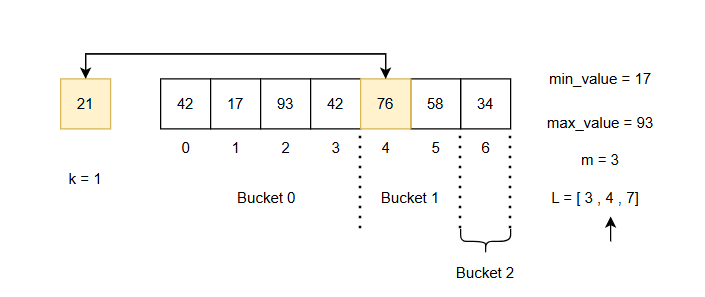
\includegraphics[width=0.7\textwidth]{img/flash_sort/7.png}
        \caption{Minh họa FlashSort-7}
    \end{figure}
    
    \begin{figure}[H]
        \centering
        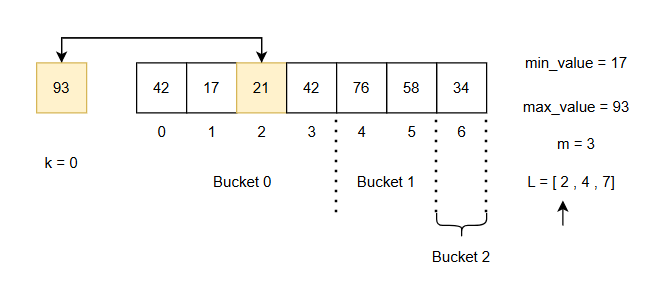
\includegraphics[width=0.7\textwidth]{img/flash_sort/8.png}
        \caption{Minh họa FlashSort-8}
    \end{figure}
    
    \begin{figure}[H]
        \centering
        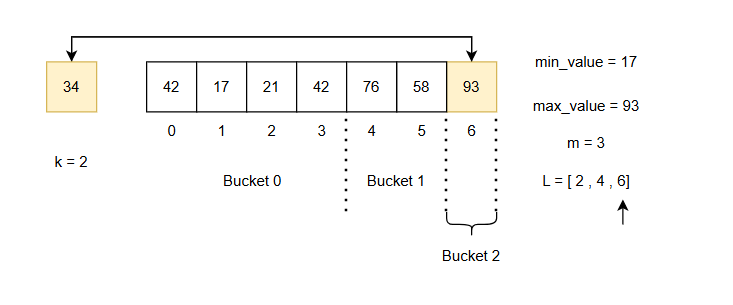
\includegraphics[width=0.7\textwidth]{img/flash_sort/9.png}
        \caption{Minh họa FlashSort-9}
    \end{figure}
    
    \begin{figure}[H]
        \centering
        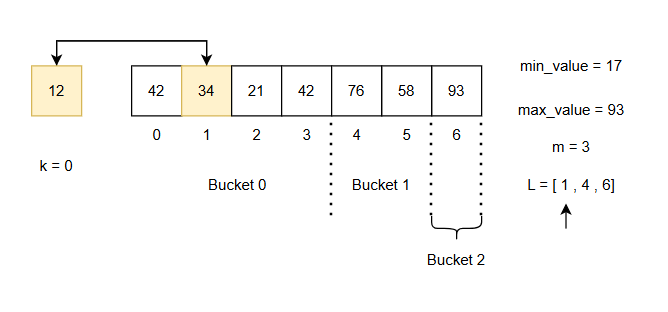
\includegraphics[width=0.7\textwidth]{img/flash_sort/10.png}
        \caption{Minh họa FlashSort-10}
    \end{figure}

    \begin{figure}[H]
        \centering
        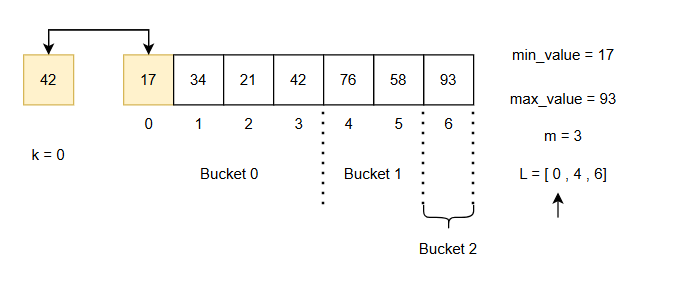
\includegraphics[width=0.7\textwidth]{img/flash_sort/11.png}
        \caption{Minh họa FlashSort-11}
    \end{figure}

    \item Hoàn thành bước phân phối, sau đó ta thực hiện Insertion Sort trên từng Bucket:
    \begin{figure}[H]
        \centering
        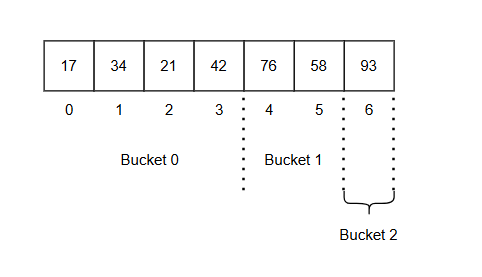
\includegraphics[width=0.7\textwidth]{img/flash_sort/12.png}
        \caption{Minh họa FlashSort-12}
    \end{figure}

    \item Hoành thành sắp xếp:
    \begin{figure}[H]
        \centering
        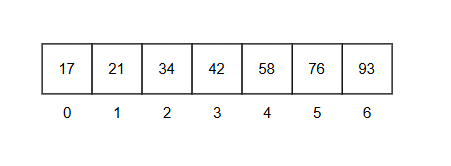
\includegraphics[width=0.7\textwidth]{img/flash_sort/13.png}
        \caption{Minh họa FlashSort-13}
    \end{figure}
\end{enumerate}

\subsubsection{Độ phức tạp}
\begin{itemize}
    \item[\textbf{--}] \textbf{Thời gian:}
    \begin{itemize}
        \item[$\bullet$] \textbf{Best Case:} \(\mathcal{O}(n)\), xảy ra khi mảng đã được phân bố đồng đều hoặc có cấu trúc dễ dàng phân nhóm. Trong trường hợp này, thuật toán có thể phân loại mảng trong một lần quét mà không cần phải thực hiện bất kỳ phép hoán đổi nào.
        \item[$\bullet$] \textbf{Average Case:} \(\mathcal{O}(n + k)\), độ phức tạp này thường thấy khi dữ liệu được phân bố ngẫu nhiên. Trong trường hợp này, Flash Sort sử dụng một phương pháp phân vùng và sắp xếp các phần tử trong các nhóm.
        \item[$\bullet$] \textbf{Worst Case:} \(\mathcal{O}(n^2)\), xảy ra khi dữ liệu có phân bố bất lợi hoặc có sự phân bố không đều giữa các giá trị. Trong trường hợp này, Flash Sort sẽ cần phải thực hiện các phép hoán đổi nhiều hơn.
    \end{itemize}
    \item[\textbf{--}] \textbf{Không gian:}
    \begin{itemize}
        \item[$\bullet$] Flash Sort yêu cầu một mảng phụ để lưu trữ các chỉ số phân loại (buckets). Kích thước của mảng phụ này phụ thuộc vào số lượng phần tử trong mảng gốc và số lượng buckets được sử dụng. Cụ thể, nếu ta có \(n\) phần tử và \(m\) buckets, thì độ phức tạp bộ nhớ của Flash Sort là:
        \[
        \mathcal{O}(n + m)
        \]
        \item[$\bullet$] Mảng gốc: \(\mathcal{O}(n)\)
        \item[$\bullet$] Mảng phụ (buckets): \(\mathcal{O}(m)\)
        \item[$\bullet$] Trong trường hợp tốt nhất, số lượng buckets \(m\) có thể nhỏ hơn hoặc bằng số lượng phần tử \(n\), do đó độ phức tạp bộ nhớ có thể được coi là \(\mathcal{O}(n)\).
        \item[$\bullet$] Trong trường hợp xấu nhất, số lượng buckets \(m\) có thể lớn hơn, dẫn đến độ phức tạp bộ nhớ là \(\mathcal{O}(n + m)\).
    \end{itemize}
    \item[\textbf{--}] \textbf{Tính ổn định:}
    \begin{itemize}
        \item[$\bullet$] Flash Sort là một thuật toán \textbf{không ổn định}. Điều này có nghĩa là khi hai phần tử có giá trị bằng nhau, thứ tự ban đầu của chúng có thể thay đổi trong quá trình sắp xếp.
    \end{itemize}
\end{itemize}
